\documentclass[12pt,a4paper]{article}
\usepackage[utf8]{inputenc}
\usepackage[utf8]{vietnam}
\usepackage{amsmath}
\usepackage{amsfonts}
\usepackage{amssymb}
\usepackage{graphicx}
\graphicspath{{images/}}
\usepackage[left=2cm,right=2cm,top=2cm,bottom=2cm]{geometry}
\begin{document}
    \begin{enumerate}
        \item[] \textbf{Lưu ý: Trong mỗi trường hợp tính toán xong nên vẽ hình để làm quen với cách vẽ hình (chỉ vẽ hình trên mặt bằng)}
        \item Cho căn nhà có kích thước như hình, tại  $A$ và $B$ người ta đặt 2 kim thu sét có độ cao bằng nhau và bằng $5m$. Vẽ vùng bảo vệ, cho biết căn nhà có được bảo vệ hoàn toàn không?
            \begin{figure}[htp]
                \begin{center}
                    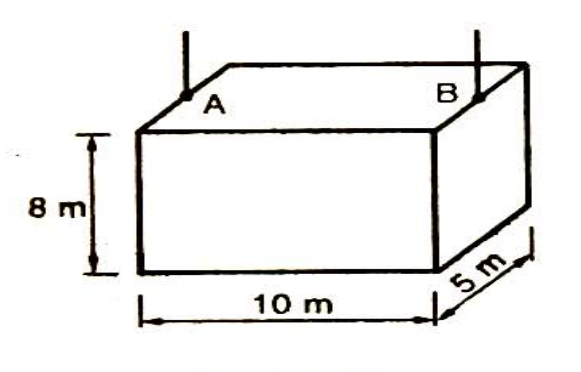
\includegraphics[scale=.4]{baitap1}
                \end{center}
            \end{figure}
            
        \item Cho căn nhà có kích thước như hình, tại  $A$ và $B$ người ta đặt 2 kim thu sét có độ cao $6m$ và $3m$. Vẽ vùng bảo vệ, cho biết khả năng bảo vệ của 2 kim thu sét?
            \begin{figure}[htp]
                \begin{center}
                    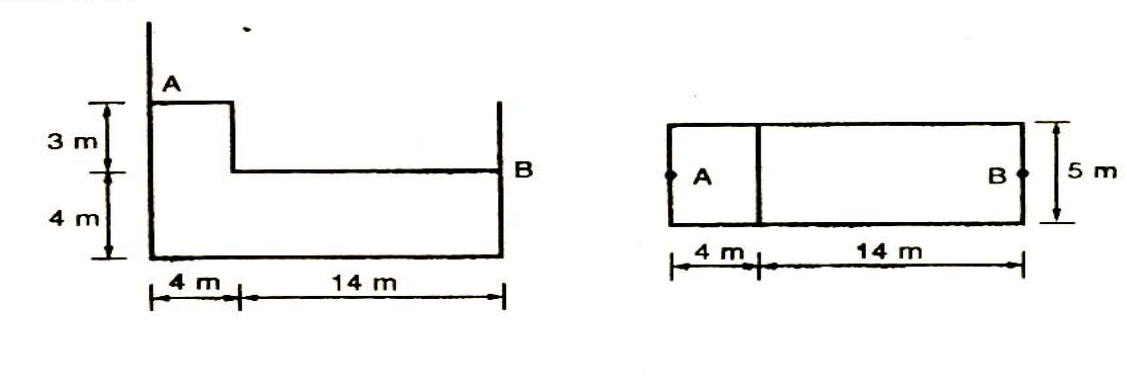
\includegraphics[scale=.4]{baitap2}
                \end{center}
            \end{figure}
            
        \item Cho căn nhà có kích thước như hình, người ta đặt 3 kim thu sét bằng nhau tại các vị trí 1, 2, 3 và bằng $4m$. Hỏi căn nhà có được bảo vệ toàn bộ hay không?
            \begin{figure}[htp]
                \begin{center}
                    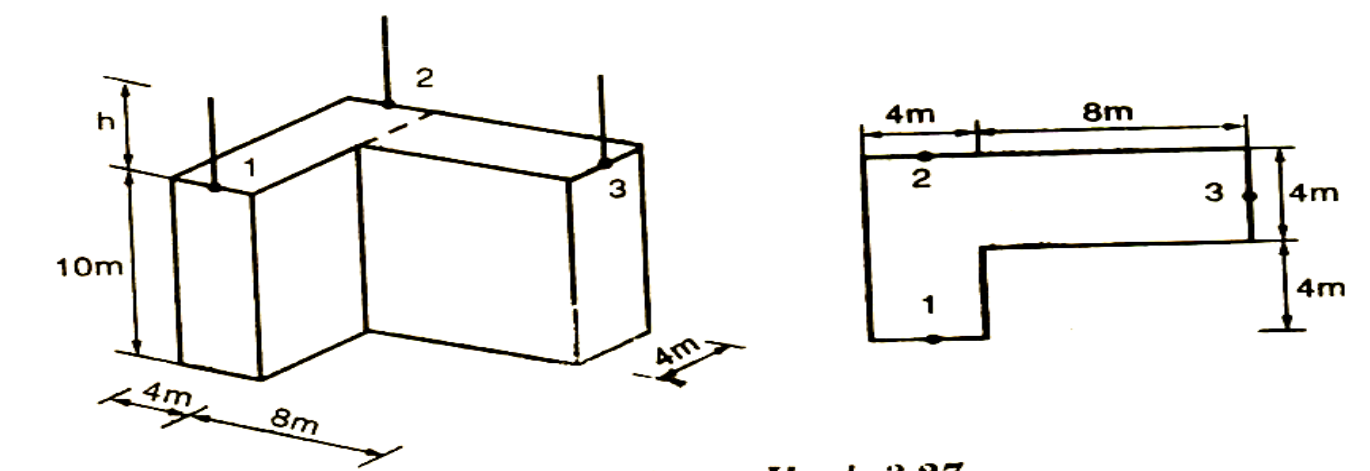
\includegraphics[scale=.35]{baitap3}
                \end{center}
            \end{figure} 
        
        \item Cho căn nhà có kích thước như hình, người ta đặt 3 kim thu sét bằng nhau tại các vị trí 1, 2, 3 và bằng $h$. Tìm độ cao $h$ nhỏ nhất để có thể bảo vệ toàn bộ căn nhà?
            \begin{figure}[htp]
                \begin{center}
                    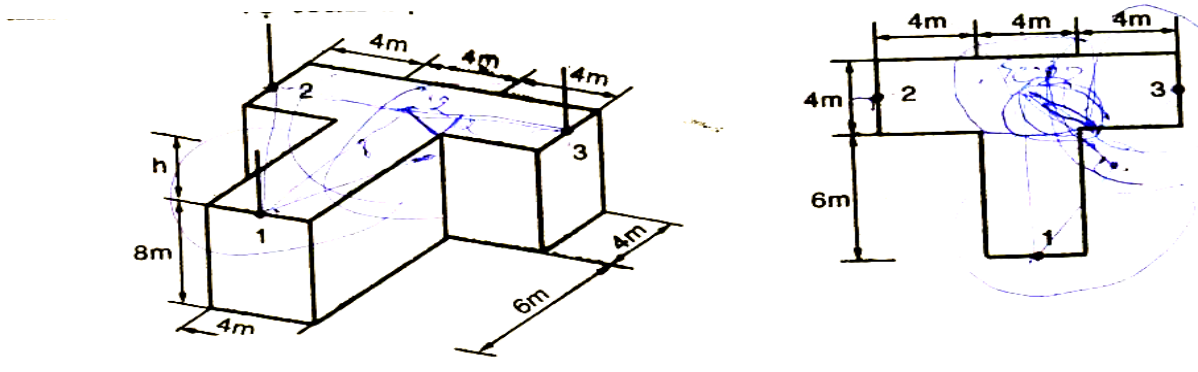
\includegraphics[scale=.35]{baitap4}
                \end{center}
            \end{figure}
            
        \item Cho căn nhà có kích thước như hình, người ta đặt 3 kim thu sét bằng nhau tại các vị trí 1, 2, 3 và bằng $h$. Tìm độ cao $h$ nhỏ nhất để có thể bảo vệ toàn bộ căn nhà?
            \begin{figure}[htp]
                \begin{center}
                    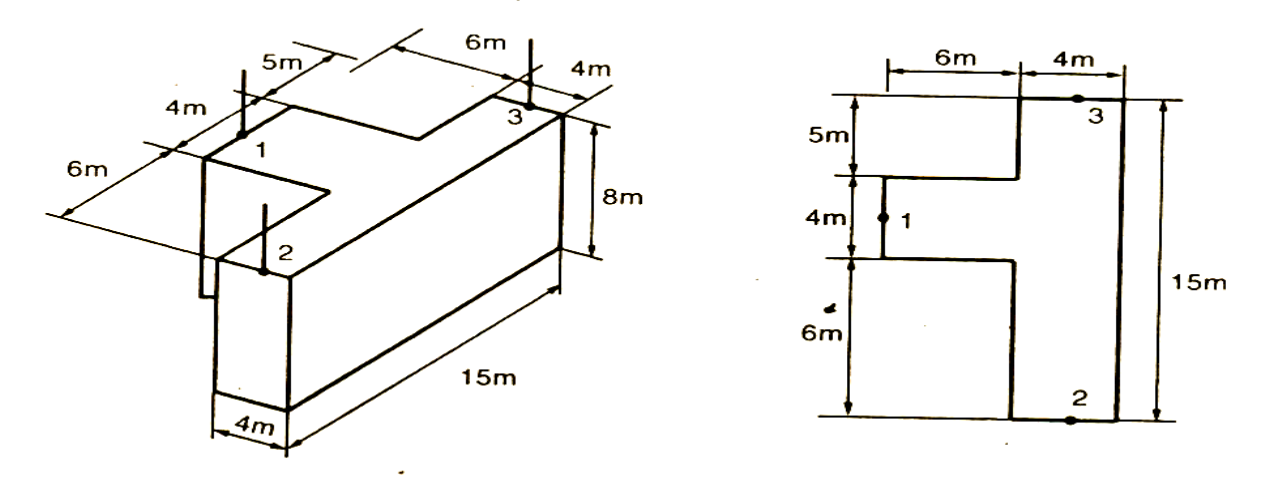
\includegraphics[scale=.35]{baitap5}
                \end{center}
            \end{figure}
            
        \item Cho căn nhà có kích thước như hình, người ta đặt 3 kim thu sét bằng nhau tại các vị trí $a, b, c, d$ và bằng $4m$. Hỏi căn nhà có được bảo vệ toàn bộ hay không?
            \begin{figure}[htp]
                \begin{center}
                    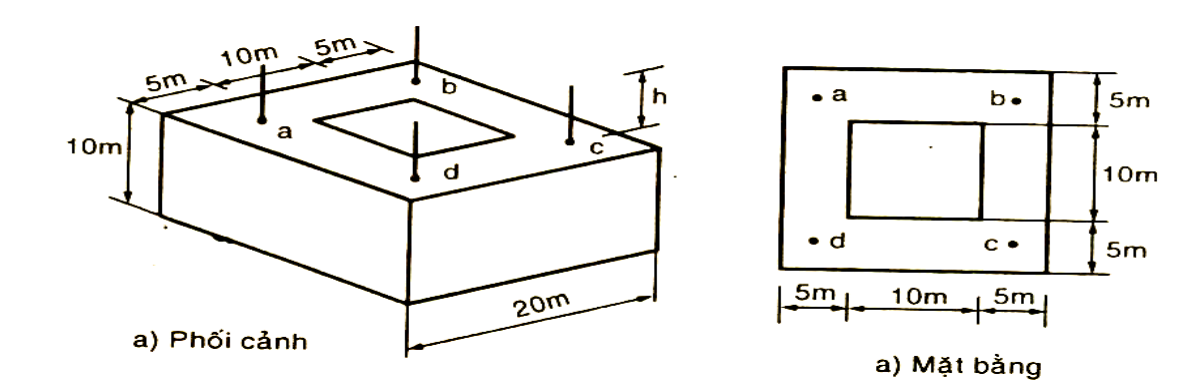
\includegraphics[scale=.4]{baitap6}
                \end{center}
            \end{figure}

        \item Cho căn nhà có kích thước như hình trong bài tập 6, người ta đặt 4 kim thu sét bằng nhau tại các vị trí $a, b, c, d$ và bằng $h$. Tìm độ cao $h$ nhỏ nhất để có thể bảo vệ toàn bộ căn nhà?            
    \end{enumerate}
\end{document}